\section{Bread and Butter}
\label{sec:bnb}

\subsection{Low Percent}

\clearpage
\subsection{dtilt $\rightarrow$ RCBG}

\begin{figure}[h]
    \centering
    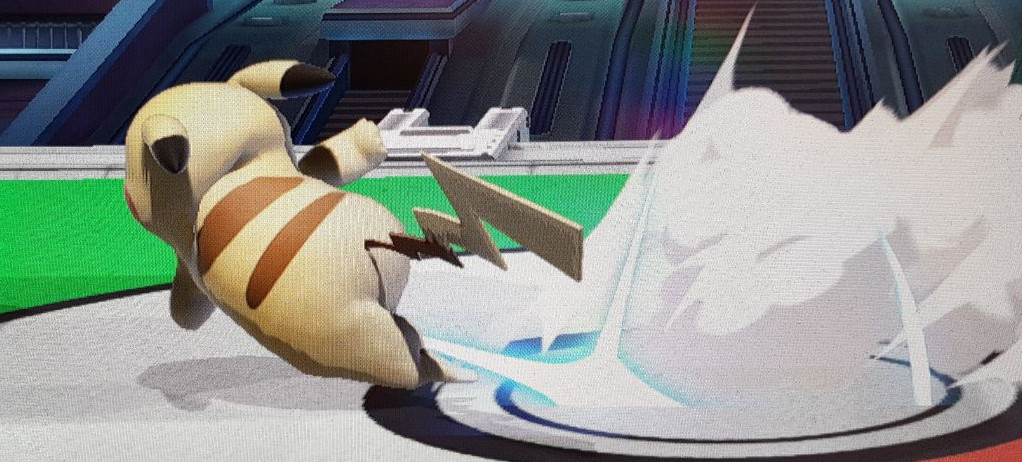
\includegraphics[width=.6\linewidth]{images/pika-rcbg}
    \caption{Successful execution of RCBG. Notice the blue flash.}
    \label{fig:pika-rcbg}
\end{figure}

Depending on character, rage, execution, and spacing, down-tilt can true combo
into a grab.

A RCBG (roll cancel boost grab) can  reach  farther than dash grab in the same
amount of time, and is  performed  by  first  dashing,  then  shielding,  then
pressing A, in quick succession. Pikachu will appear to do a dash grab, but if
performed successfully, a blue flash will appear, indicating that the roll was
cancelled (see figure \ref{fig:pika-rcbg}).

%\todo[inline]{Add screenshot showing blue flash}

Executing  a perfect RCBG reliably is difficult (dash frame 1, shield frame 2,
A on frame 3) and it reaches the shortest distance. The more you wait  between
the inputs, the farther your grab will  reach,  but  the  later you will grab.
Table \ref{tab:rcbg-frame-data} lists how the distance and grab speed  changes
depending on execution.

It is currently unclear whether perfect  execution of RCBG is requried for the
upper  range  of  percents,  or whether some characters require you to  do  an
``imperfect'' RCBG  on  purpose to cover the necessary distance. The following
tables  show  ranges  that are possible, but note that for  the  upper  ranges
execution is much tighter and possibly more nuanced than for the lower ranges.

Also note that these percents were obtained from unspaced dtilt. A well spaced
dtilt may decrease the upper range where this works.

\begin{table}[h]
    \centering
    \caption{Comparison of frame data between RCBG and Dash grab}
    \begin{subtable}[t]{.45\linewidth}
        \centering
        \caption{Roll cancel boost grab}
        \begin{tabular}{ccc|cc}
            \toprule
            \textbf{Dash} & \textbf{Shield} & \textbf{A} & \textbf{Grabbox} & \textbf{Distance} \\
            \midrule
            1 & 2 & 3 & 13 & 2.7 \\
            1 & 2 & 4 & 14 & 2.9 \\
            1 & 3 & 4 & 14 & 2.9 \\
            1 & 2 & 5 & 15 & 3.1 \\
            1 & 4 & 7 & 17 & 3.4 \\
            1 & 5 & 8 & 18 & 3.7 \\
            \bottomrule
        \end{tabular}
        \label{tab:rcbg-frame-data}
    \end{subtable}
    \begin{subtable}[t]{.45\linewidth}
        \centering
        \caption{Dash Grab}
        \begin{tabular}{cc|cc}
            \toprule
            \textbf{Dash} & \textbf{Grab} & \textbf{Grabbox} & \textbf{Distance} \\
            \midrule
            1 & 2 & 12 & 2.2 \\
            1 & 3 & 13 & 2.4 \\
            1 & 4 & 14 & 2.6 \\
            1 & 5 & 15 & 2.8 \\
            \bottomrule
        \end{tabular}
        \label{tab:dashgrab-frame-data}
    \end{subtable}
\end{table}

\begin{table}[h]
    \centering
    \caption{Rage}
    \begin{tabular}{ccc}
        \toprule
        \textbf{Rage} & \textbf{Lower} & \textbf{Upper} \\
        \midrule
        $50\%$  & $+1$ & $-2$ \\
        $100\%$ & $+4$ & $-6$ \\
        $150\%$ & $+8$ & $-11$ \\
        \bottomrule
    \end{tabular}
\end{table}

\begin{table}[h]
    \centering
    \caption{Percent ranges for dtilt $\rightarrow$ rcbg and dtilt $\rightarrow$ dash grab. Data obtained from\cite{ref:jason:rcbg-ranges}}
    \begin{subtable}[t]{.45\linewidth}
        \centering
        \caption{}
        \begin{tabular}{lcc}
            \toprule
            \textbf{Character} & \textbf{Dash Grab} & \textbf{RCBG} \\
            \midrule
            Mario             & 38-46          & 47-53 \\
            DK                & 49             & 49-60 \\
            Link              & 39-47          & 48-60 \\
            Samus             &                & 45-48 \\
            Yoshi             & 39-47          & 48-62 \\
            Kirby             & 34-41\tnote{1} & 42-57 \\
            Fox               & 33-40\tnote{1} & 41-70 \\
            Pikachu           & 34-41\tnote{1} & 42-55 \\
            Luigi             & 38-45\tnote{2} & 42-51\tnote{3} \\
            Ness              & 37-45          & 46-55 \\
            Captain Falcon    & 39-47          & 48-58 \\
            Jigglypuff        & 31-38\tnote{1} & 39-44 \\
            Peach             & 36-43\tnote{1} & 44-49 \\
            Bowser            & 47-55          & 56-75 \\
            Ice climbers      &                &       \\
            Sheik             & 33-40\tnote{1} & 41-55 \\
            Zelda             & 35-42          & 43-53 \\
            Dr. Mario         & 38-46\tnote{1} & 47-55 \\
            Pichu             & 30-36\tnote{1} & 37-51 \\
            Falco             & 34-41\tnote{1} & 42-57 \\
            Marth             & 35-44          & 45-54 \\
            Young link        & 36-43          & 44-57 \\
            Ganondorf         & 42-51          & 52-73 \\
            Mewtwo            & 34-41          & 42-53 \\
            Roy               & 37-45          & 46-57 \\
            Game and Watch    & 33-40          & 41-54 \\
            Meta Knight       & 34-41          & 42-54 \\
            Pit               & 37-45          & 46-60 \\
            Zero Suit Samus   & 34-41          & 42-57 \\
            Wario             & 40-48          & 49-62 \\
            Snake             & 40-48          & 49-56 \\
            Ike               & 40-48          & 49-63 \\
            Squirtle          & 33-40\tnote{1} & 41-50\tnote{4} \\
            Ivysaur           & 37-45\tnote{1} & 46-56\tnote{5} \\
            Charizard         & 42-50\tnote{1} & 51-63\tnote{6} \\
            Diddy Kong        & 36-44          & 45-55 \\
            Lucas             & 37-45\tnote{1} & 46-54 \\
            Sonic             & 35-42          & 43-58 \\
            King Dedede       & 44-48          & 49-53 \\
            Olimar            & 34-41          & 42-48 \\
            \bottomrule
        \end{tabular}
        \begin{tablenotes}
            \item[1] Character has a frame 2 or faster option.
            \item[2] Only if they mash cyclone. Doesn't work for spotdodge.
            \item[3] 42-45 if they mash spotdodge.
            \item[4] 41-45 if mashing switch.
            \item[5] 46-52 if mashing switch.
            \item[6] 51-55 if mashing switch.
        \end{tablenotes}
    \end{subtable}
    \begin{subtable}[t]{.45\linewidth}
        \centering
        \caption{}
        \begin{tabular}{lcc}
            \toprule
            \textbf{Character} & \textbf{Dash Grab} & \textbf{RCBG} \\
            \midrule
            Lucario           & 37-44          & 45-54 \\
            R.O.B             & 40-48\tnote{1} & 49-60\tnote{3} \\
            Toon Link         &                & 41-44 \\
            Wolf              & 37-44          & 45-60 \\
            Villager          & 37-44          & 45-57 \\
            Megaman           & 39-47          & 48-53 \\
            Wii Fit Trainer   & 37-45          & 46-60 \\
            Rosalina and Luma &                & 38-41\tnote{5} \\
            Little Mac        & 35-43\tnote{1} & 44-52 \\
            Greninja          & 36-43          & 44-52 \\
            Palutena          & 36-44          & 45-55 \\
            Pac-Man           & 37-45          & 46-52 \\
            Robin             & 38-45          & 46-48 \\
            Shulk             & 38-45\tnote{2} & 46-51\tnote{2} \\
            Bowser Jr.        & 41-49          &       \\
            Duck Hunt         &                & 39-42\tnote{4} \\
            Ryu/Ken           & 39-47\tnote{1} & 48-58 \\
            Cloud             & 38-46          & 47-50 \\
            Corrin            & 38-46          & 47-57 \\
            Bayonetta         & 34-41          & 42-61 \\
            Inkling           & 37-44          & 45-56 \\
            Ridley            &                & 44-48 \\
            Richter           &                & 44-48 \\
            King K. Rool      & 45-55          & 56-72 \\
            Isabelle          & 36-43          & 44-50 \\
            Incineroar        & 42-50          & 51-70 \\
            Piranha Plant     &                & 46-49 \\
            Joker             & 37-44          & 45-60 \\
            Hero              & 39-46          & 47-61 \\
            Banjo             &                & 44-48 \\
            Terry             & 40-48          & 49-58 \\
            Byleth            & 38-45          & 46-53 \\
            Min Min           & 39-47          & 48-64 \\
            Steve             &                & 41-44 \\
            Sephiroth         & 34-41          & 42-51 \\
            Pyra              & 38-46          & 47-51 \\
            Mythra            & 37-44\tnote{1} & 45-63 \\
            Mii Swordfighter  & 38-46          & 47-58 \\
            Mii Gunner        & 39-47          &       \\
            Mii Brawler       & 37-45\tnote{1} & 46-65 \\
            \bottomrule
        \end{tabular}
        \begin{tablenotes}
            \item[1] Character has a frame 2 or faster option.
            \item[2] Character is cheating.
            \item[3] Doesn't work if they up-b.
            \item[4] Doesn't work if they mash can.
            \item[5] Idk how luma works
        \end{tablenotes}
    \end{subtable}
\end{table}

